
Como primer resultado de esta investigación se ha consolidado una base de datos georreferenciada de indicadores socio-económicos y variables físicas relacionadas a la identificación
de zonas de interés para la implementación de soluciones de energía alternativa usando recursos de biomasa y solar.  Las capas procesadas se recogieron en un
único formato geopackage, formato soportado por la OGC como estandar interoperable, que contiene el total de total de los indicadores mencionados en la sección
\ref{sec:fuentes}.  El archivo se distribuye con este informe como un anexo digital.

Indice de potencialidad
\begin{figure}
    \centering
    \includegraphics[width=0.8\textwidth]{figures/indice}
    \caption{Indice de potencialidad propuesto.}
    \label{fig:indice}
\end{figure}

Agregación por municipios
\begin{figure}
    \centering
    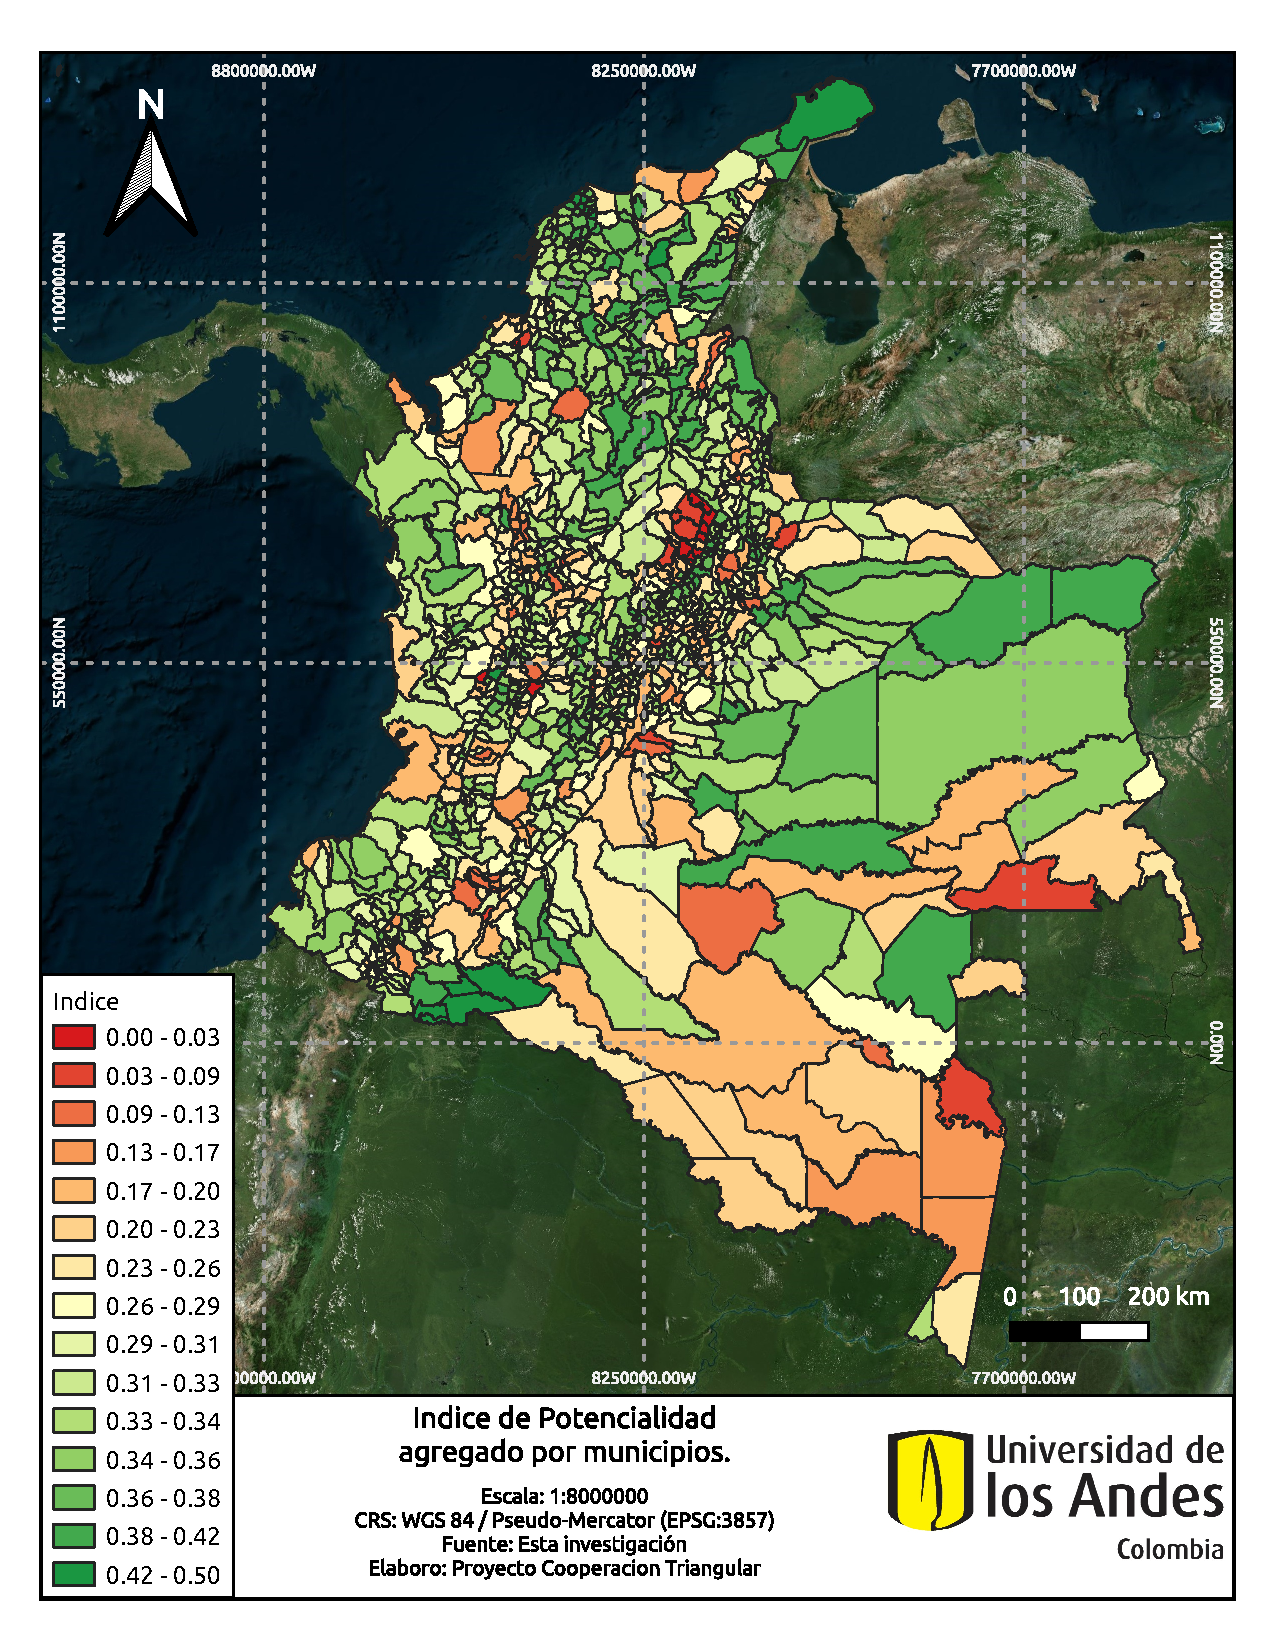
\includegraphics[width=0.8\textwidth]{figures/pormunicipios}
    \caption{Indice de potencialidad agregado por municipios.}
    \label{fig:pormunicipios}
\end{figure}

Filtrado por municipios PDET
\begin{figure}
    \centering
    \includegraphics[width=0.8\textwidth]{figures/porpdet}
    \caption{Indice de potencialidad filtrado por municipio PDET.}
    \label{fig:porpdet}
\end{figure}

Modelo QGIS con la implementación de la metodología.
\begin{figure}
    \centering
    \includegraphics[angle=90, width=0.56\textwidth]{figures/modelo}
    \caption{Modelo QGIS con la implementación de la metodología.}
    \label{fig:modelo}
\end{figure}

Conclusión: listado de municipios con alto potencial.

Resultados.
Mostrar mapa final. Y una tabla con los primeros 10 municipios. Justificación de los pesos seleccionados con base en los objetivos del proyecto.

Conclusiones.
Indicar cuál es la zona seleccionada que será utilizada para las siguientes fases del proyecto. Sobre está zona se hará el estudio de concepto. Describir
brevemente lo que se hará.
Metodología parametrizable para la priorización/selección de la zona bajo estudio.
Posibilidad de incluir otros indicadores, tanto socio económicos como físicos, en estudios posteriores con base en los objetivos del proyecto.
Importante la disponibilidad de datos abiertos de fuentes oficiales.
